% Options for packages loaded elsewhere
\PassOptionsToPackage{unicode}{hyperref}
\PassOptionsToPackage{hyphens}{url}
%
\documentclass[
]{article}
\usepackage{amsmath,amssymb}
\usepackage{iftex}
\ifPDFTeX
  \usepackage[T1]{fontenc}
  \usepackage[utf8]{inputenc}
  \usepackage{textcomp} % provide euro and other symbols
\else % if luatex or xetex
  \usepackage{unicode-math} % this also loads fontspec
  \defaultfontfeatures{Scale=MatchLowercase}
  \defaultfontfeatures[\rmfamily]{Ligatures=TeX,Scale=1}
\fi
\usepackage{lmodern}
\ifPDFTeX\else
  % xetex/luatex font selection
\fi
% Use upquote if available, for straight quotes in verbatim environments
\IfFileExists{upquote.sty}{\usepackage{upquote}}{}
\IfFileExists{microtype.sty}{% use microtype if available
  \usepackage[]{microtype}
  \UseMicrotypeSet[protrusion]{basicmath} % disable protrusion for tt fonts
}{}
\makeatletter
\@ifundefined{KOMAClassName}{% if non-KOMA class
  \IfFileExists{parskip.sty}{%
    \usepackage{parskip}
  }{% else
    \setlength{\parindent}{0pt}
    \setlength{\parskip}{6pt plus 2pt minus 1pt}}
}{% if KOMA class
  \KOMAoptions{parskip=half}}
\makeatother
\usepackage{xcolor}
\usepackage[margin=1in]{geometry}
\usepackage{color}
\usepackage{fancyvrb}
\newcommand{\VerbBar}{|}
\newcommand{\VERB}{\Verb[commandchars=\\\{\}]}
\DefineVerbatimEnvironment{Highlighting}{Verbatim}{commandchars=\\\{\}}
% Add ',fontsize=\small' for more characters per line
\usepackage{framed}
\definecolor{shadecolor}{RGB}{248,248,248}
\newenvironment{Shaded}{\begin{snugshade}}{\end{snugshade}}
\newcommand{\AlertTok}[1]{\textcolor[rgb]{0.94,0.16,0.16}{#1}}
\newcommand{\AnnotationTok}[1]{\textcolor[rgb]{0.56,0.35,0.01}{\textbf{\textit{#1}}}}
\newcommand{\AttributeTok}[1]{\textcolor[rgb]{0.13,0.29,0.53}{#1}}
\newcommand{\BaseNTok}[1]{\textcolor[rgb]{0.00,0.00,0.81}{#1}}
\newcommand{\BuiltInTok}[1]{#1}
\newcommand{\CharTok}[1]{\textcolor[rgb]{0.31,0.60,0.02}{#1}}
\newcommand{\CommentTok}[1]{\textcolor[rgb]{0.56,0.35,0.01}{\textit{#1}}}
\newcommand{\CommentVarTok}[1]{\textcolor[rgb]{0.56,0.35,0.01}{\textbf{\textit{#1}}}}
\newcommand{\ConstantTok}[1]{\textcolor[rgb]{0.56,0.35,0.01}{#1}}
\newcommand{\ControlFlowTok}[1]{\textcolor[rgb]{0.13,0.29,0.53}{\textbf{#1}}}
\newcommand{\DataTypeTok}[1]{\textcolor[rgb]{0.13,0.29,0.53}{#1}}
\newcommand{\DecValTok}[1]{\textcolor[rgb]{0.00,0.00,0.81}{#1}}
\newcommand{\DocumentationTok}[1]{\textcolor[rgb]{0.56,0.35,0.01}{\textbf{\textit{#1}}}}
\newcommand{\ErrorTok}[1]{\textcolor[rgb]{0.64,0.00,0.00}{\textbf{#1}}}
\newcommand{\ExtensionTok}[1]{#1}
\newcommand{\FloatTok}[1]{\textcolor[rgb]{0.00,0.00,0.81}{#1}}
\newcommand{\FunctionTok}[1]{\textcolor[rgb]{0.13,0.29,0.53}{\textbf{#1}}}
\newcommand{\ImportTok}[1]{#1}
\newcommand{\InformationTok}[1]{\textcolor[rgb]{0.56,0.35,0.01}{\textbf{\textit{#1}}}}
\newcommand{\KeywordTok}[1]{\textcolor[rgb]{0.13,0.29,0.53}{\textbf{#1}}}
\newcommand{\NormalTok}[1]{#1}
\newcommand{\OperatorTok}[1]{\textcolor[rgb]{0.81,0.36,0.00}{\textbf{#1}}}
\newcommand{\OtherTok}[1]{\textcolor[rgb]{0.56,0.35,0.01}{#1}}
\newcommand{\PreprocessorTok}[1]{\textcolor[rgb]{0.56,0.35,0.01}{\textit{#1}}}
\newcommand{\RegionMarkerTok}[1]{#1}
\newcommand{\SpecialCharTok}[1]{\textcolor[rgb]{0.81,0.36,0.00}{\textbf{#1}}}
\newcommand{\SpecialStringTok}[1]{\textcolor[rgb]{0.31,0.60,0.02}{#1}}
\newcommand{\StringTok}[1]{\textcolor[rgb]{0.31,0.60,0.02}{#1}}
\newcommand{\VariableTok}[1]{\textcolor[rgb]{0.00,0.00,0.00}{#1}}
\newcommand{\VerbatimStringTok}[1]{\textcolor[rgb]{0.31,0.60,0.02}{#1}}
\newcommand{\WarningTok}[1]{\textcolor[rgb]{0.56,0.35,0.01}{\textbf{\textit{#1}}}}
\usepackage{longtable,booktabs,array}
\usepackage{calc} % for calculating minipage widths
% Correct order of tables after \paragraph or \subparagraph
\usepackage{etoolbox}
\makeatletter
\patchcmd\longtable{\par}{\if@noskipsec\mbox{}\fi\par}{}{}
\makeatother
% Allow footnotes in longtable head/foot
\IfFileExists{footnotehyper.sty}{\usepackage{footnotehyper}}{\usepackage{footnote}}
\makesavenoteenv{longtable}
\usepackage{graphicx}
\makeatletter
\def\maxwidth{\ifdim\Gin@nat@width>\linewidth\linewidth\else\Gin@nat@width\fi}
\def\maxheight{\ifdim\Gin@nat@height>\textheight\textheight\else\Gin@nat@height\fi}
\makeatother
% Scale images if necessary, so that they will not overflow the page
% margins by default, and it is still possible to overwrite the defaults
% using explicit options in \includegraphics[width, height, ...]{}
\setkeys{Gin}{width=\maxwidth,height=\maxheight,keepaspectratio}
% Set default figure placement to htbp
\makeatletter
\def\fps@figure{htbp}
\makeatother
\setlength{\emergencystretch}{3em} % prevent overfull lines
\providecommand{\tightlist}{%
  \setlength{\itemsep}{0pt}\setlength{\parskip}{0pt}}
\setcounter{secnumdepth}{-\maxdimen} % remove section numbering
\ifLuaTeX
  \usepackage{selnolig}  % disable illegal ligatures
\fi
\IfFileExists{bookmark.sty}{\usepackage{bookmark}}{\usepackage{hyperref}}
\IfFileExists{xurl.sty}{\usepackage{xurl}}{} % add URL line breaks if available
\urlstyle{same}
\hypersetup{
  pdftitle={6.27 숙제 markdown},
  hidelinks,
  pdfcreator={LaTeX via pandoc}}

\title{6.27 숙제 markdown}
\author{}
\date{\vspace{-2.5em}2023-06-30}

\begin{document}
\maketitle

\hypertarget{uxc219uxc81c}{%
\section{숙제}\label{uxc219uxc81c}}

\hypertarget{section}{%
\subsection{\#\#6.27}\label{section}}

Packages

\begin{Shaded}
\begin{Highlighting}[]
\FunctionTok{library}\NormalTok{(tidyverse)}
\end{Highlighting}
\end{Shaded}

\begin{verbatim}
## -- Attaching core tidyverse packages ------------------------ tidyverse 2.0.0 --
## v dplyr     1.1.2     v readr     2.1.4
## v forcats   1.0.0     v stringr   1.5.0
## v ggplot2   3.4.2     v tibble    3.2.1
## v lubridate 1.9.2     v tidyr     1.3.0
## v purrr     1.0.1     
## -- Conflicts ------------------------------------------ tidyverse_conflicts() --
## x dplyr::filter() masks stats::filter()
## x dplyr::lag()    masks stats::lag()
## i Use the conflicted package (<http://conflicted.r-lib.org/>) to force all conflicts to become errors
\end{verbatim}

\begin{Shaded}
\begin{Highlighting}[]
\FunctionTok{library}\NormalTok{(ggplot2)}
\FunctionTok{library}\NormalTok{(NonCompart)}
\FunctionTok{library}\NormalTok{ (knitr)}
\end{Highlighting}
\end{Shaded}

Raw Data

\begin{Shaded}
\begin{Highlighting}[]
\NormalTok{data }\OtherTok{\textless{}{-}}   \FunctionTok{read\_csv}\NormalTok{(}\StringTok{"pkpd\_dataset.csv"}\NormalTok{, }\AttributeTok{na=} \StringTok{"NA"}\NormalTok{)}
\end{Highlighting}
\end{Shaded}

\begin{verbatim}
## Rows: 20820 Columns: 21
## -- Column specification --------------------------------------------------------
## Delimiter: ","
## chr  (4): TIMEUNIT, NAME, EVENTU, TRTACT
## dbl (17): ID, TIME, NOMTIME, AMT, LIDV, CMT, CENS, EVID, WEIGHTB, eff0, DOSE...
## 
## i Use `spec()` to retrieve the full column specification for this data.
## i Specify the column types or set `show_col_types = FALSE` to quiet this message.
\end{verbatim}

\hypertarget{section-1}{%
\subsubsection{1}\label{section-1}}

Data

\begin{Shaded}
\begin{Highlighting}[]
\NormalTok{data\_cycle\_1 }\OtherTok{\textless{}{-}}\NormalTok{ data }\SpecialCharTok{|\textgreater{}}
  \FunctionTok{filter}\NormalTok{(CMT }\SpecialCharTok{==} \DecValTok{2} \SpecialCharTok{\&}\NormalTok{ CYCLE }\SpecialCharTok{==} \DecValTok{1} \SpecialCharTok{\&}\NormalTok{ NAME }\SpecialCharTok{==} \StringTok{"PK Concentration"}\NormalTok{) }\SpecialCharTok{|\textgreater{}}
  \FunctionTok{select}\NormalTok{(ID, NOMTIME, LIDV, DOSE) }\SpecialCharTok{|\textgreater{}}
  \FunctionTok{mutate}\NormalTok{(}\AttributeTok{DOSE =} \FunctionTok{as.factor}\NormalTok{(DOSE))}
\end{Highlighting}
\end{Shaded}

Plot: cycle1 cmt2 pk

\begin{Shaded}
\begin{Highlighting}[]
\NormalTok{data\_cycle\_1 }\SpecialCharTok{|\textgreater{}}
  \FunctionTok{ggplot}\NormalTok{(}\FunctionTok{aes}\NormalTok{(}\AttributeTok{x =}\NormalTok{ NOMTIME, }\AttributeTok{y =}\NormalTok{ LIDV, }\AttributeTok{color =}\NormalTok{ DOSE, }\AttributeTok{group =}\NormalTok{ ID)) }\SpecialCharTok{+} \FunctionTok{geom\_line}\NormalTok{() }\SpecialCharTok{+}
  \FunctionTok{geom\_point}\NormalTok{() }\SpecialCharTok{+} \FunctionTok{facet\_wrap}\NormalTok{(}\SpecialCharTok{\textasciitilde{}}\NormalTok{DOSE) }\SpecialCharTok{+} \FunctionTok{labs}\NormalTok{(}\AttributeTok{title =} \StringTok{"cycle1\_cmt2\_pk"}\NormalTok{)}
\end{Highlighting}
\end{Shaded}

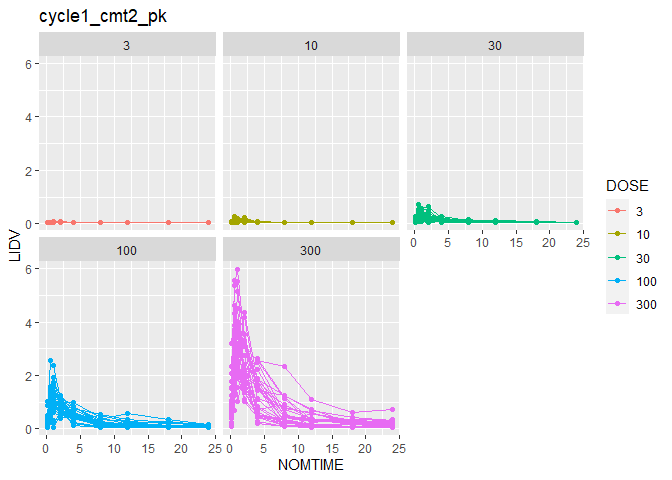
\includegraphics{6.27-Markdown_files/figure-latex/unnamed-chunk-4-1.pdf}

\begin{Shaded}
\begin{Highlighting}[]
\FunctionTok{ggsave}\NormalTok{(}\StringTok{\textquotesingle{}cycle1\_cmt2\_pk.png\textquotesingle{}}\NormalTok{)}
\end{Highlighting}
\end{Shaded}

\begin{verbatim}
## Saving 6.5 x 4.5 in image
\end{verbatim}

\hypertarget{section-2}{%
\subsubsection{2}\label{section-2}}

Data

\begin{Shaded}
\begin{Highlighting}[]
\NormalTok{ data\_mean\_sd }\OtherTok{\textless{}{-}}\NormalTok{ data }\SpecialCharTok{|\textgreater{}}
  \FunctionTok{filter}\NormalTok{(CYCLE }\SpecialCharTok{==} \DecValTok{1} \SpecialCharTok{\&}\NormalTok{ NAME }\SpecialCharTok{==} \StringTok{"PK Concentration"}\NormalTok{) }\SpecialCharTok{|\textgreater{}}
  \FunctionTok{select}\NormalTok{(ID, NOMTIME, LIDV, NAME, DOSE) }\SpecialCharTok{|\textgreater{}}
  \FunctionTok{mutate}\NormalTok{(}\AttributeTok{DOSE =} \FunctionTok{as.numeric}\NormalTok{(DOSE))}

\NormalTok{data\_mean\_sd\_1 }\OtherTok{\textless{}{-}}\NormalTok{ data\_mean\_sd}\SpecialCharTok{|\textgreater{}}
  \FunctionTok{group\_by}\NormalTok{(DOSE, NOMTIME) }\SpecialCharTok{|\textgreater{}}
   \FunctionTok{summarize}\NormalTok{(}\AttributeTok{LIDV\_mean =} \FunctionTok{mean}\NormalTok{(LIDV),}
             \AttributeTok{LIDV\_sd =} \FunctionTok{sd}\NormalTok{(LIDV)}
\NormalTok{            )}
\end{Highlighting}
\end{Shaded}

\begin{verbatim}
## `summarise()` has grouped output by 'DOSE'. You can override using the
## `.groups` argument.
\end{verbatim}

plot : cycle1 mean, SD pk

\begin{Shaded}
\begin{Highlighting}[]
\NormalTok{data\_mean\_sd\_1 }\SpecialCharTok{|\textgreater{}}
  \FunctionTok{ggplot}\NormalTok{(}\FunctionTok{aes}\NormalTok{(}\AttributeTok{x =}\NormalTok{ NOMTIME, }\AttributeTok{y =}\NormalTok{ LIDV\_mean)) }\SpecialCharTok{+} \FunctionTok{geom\_line}\NormalTok{() }\SpecialCharTok{+} \FunctionTok{geom\_point}\NormalTok{() }\SpecialCharTok{+}
  \FunctionTok{geom\_errorbar}\NormalTok{(}\FunctionTok{aes}\NormalTok{(}\AttributeTok{ymin =}\NormalTok{ LIDV\_mean }\SpecialCharTok{+}\NormalTok{ LIDV\_sd, }\AttributeTok{ymax =}\NormalTok{ LIDV\_mean }\SpecialCharTok{{-}}\NormalTok{ LIDV\_sd)) }\SpecialCharTok{+}
  \FunctionTok{facet\_wrap}\NormalTok{(}\SpecialCharTok{\textasciitilde{}}\NormalTok{DOSE) }\SpecialCharTok{+} \FunctionTok{labs}\NormalTok{(}\AttributeTok{title =} \StringTok{"cycle1\_pk\_mean\&sd"}\NormalTok{)}
\end{Highlighting}
\end{Shaded}

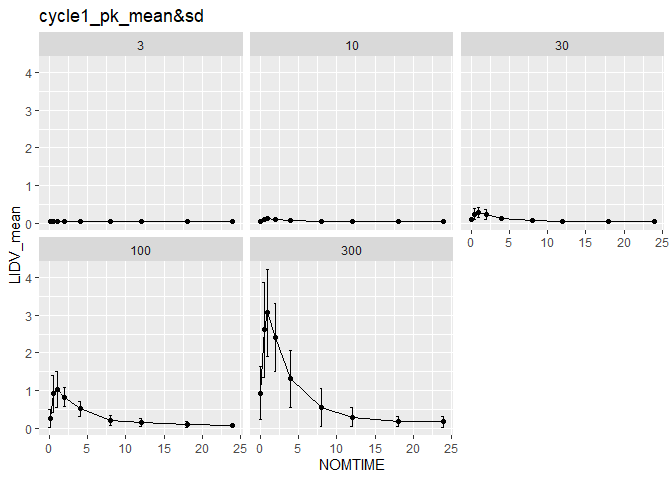
\includegraphics{6.27-Markdown_files/figure-latex/unnamed-chunk-6-1.pdf}

\begin{Shaded}
\begin{Highlighting}[]
\FunctionTok{ggsave}\NormalTok{(}\StringTok{\textquotesingle{}cycle1\_pk\_mean\&sd.png\textquotesingle{}}\NormalTok{)}
\end{Highlighting}
\end{Shaded}

\begin{verbatim}
## Saving 6.5 x 4.5 in image
\end{verbatim}

\hypertarget{section-3}{%
\subsubsection{3}\label{section-3}}

Data

\begin{Shaded}
\begin{Highlighting}[]
\NormalTok{data\_nca }\OtherTok{\textless{}{-}}\NormalTok{ data }\SpecialCharTok{|\textgreater{}}
  \FunctionTok{filter}\NormalTok{(NAME }\SpecialCharTok{==} \StringTok{"PK Concentration"} \SpecialCharTok{\&} \SpecialCharTok{!}\FunctionTok{is.na}\NormalTok{(LIDV)) }\SpecialCharTok{|\textgreater{}}
  \FunctionTok{select}\NormalTok{(ID, NOMTIME, LIDV, DOSE, NAME)}
\end{Highlighting}
\end{Shaded}

NCA result

\begin{Shaded}
\begin{Highlighting}[]
\NormalTok{nca\_result }\OtherTok{\textless{}{-}} \FunctionTok{tblNCA}\NormalTok{(data\_nca, }\AttributeTok{key=}\FunctionTok{c}\NormalTok{(}\StringTok{"ID"}\NormalTok{, }\StringTok{"DOSE"}\NormalTok{), }\AttributeTok{colTime=}\StringTok{"NOMTIME"}\NormalTok{, }\AttributeTok{colConc=}\StringTok{"LIDV"}\NormalTok{,}\AttributeTok{timeUnit =} \StringTok{"h"}\NormalTok{, }\AttributeTok{doseUnit=}\StringTok{"mg"}\NormalTok{, }\AttributeTok{concUnit=}\StringTok{"ng/mL"}\NormalTok{)}
\end{Highlighting}
\end{Shaded}

CMAX mean, median, sd, min, max

\begin{Shaded}
\begin{Highlighting}[]
\NormalTok{nca\_CMAX }\OtherTok{\textless{}{-}}\NormalTok{  nca\_result }\SpecialCharTok{|\textgreater{}}
  \FunctionTok{select}\NormalTok{(ID, DOSE, CMAX) }\SpecialCharTok{|\textgreater{}}
  \FunctionTok{group\_by}\NormalTok{(DOSE) }\SpecialCharTok{|\textgreater{}}
  \FunctionTok{summarize}\NormalTok{(}\AttributeTok{CMAX\_mean =} \FunctionTok{mean}\NormalTok{(CMAX),}
            \AttributeTok{CMAX\_median =} \FunctionTok{median}\NormalTok{(CMAX),}
            \AttributeTok{CMAX\_sd =} \FunctionTok{sd}\NormalTok{(CMAX),}
            \AttributeTok{CMAX\_min =} \FunctionTok{min}\NormalTok{(CMAX),}
            \AttributeTok{CMAX\_max =} \FunctionTok{max}\NormalTok{(CMAX)}
\NormalTok{            )}

\NormalTok{knitr}\SpecialCharTok{::}\FunctionTok{kable}\NormalTok{(nca\_CMAX)}
\end{Highlighting}
\end{Shaded}

\begin{longtable}[]{@{}rrrrrr@{}}
\toprule\noalign{}
DOSE & CMAX\_mean & CMAX\_median & CMAX\_sd & CMAX\_min & CMAX\_max \\
\midrule\noalign{}
\endhead
\bottomrule\noalign{}
\endlastfoot
3 & 0.0578545 & 0.053217 & 0.0103824 & 0.050000 & 0.087176 \\
10 & 0.1377452 & 0.130725 & 0.0454832 & 0.057579 & 0.255680 \\
30 & 0.3837983 & 0.359505 & 0.1569786 & 0.169180 & 0.902380 \\
100 & 1.4239993 & 1.399200 & 0.3964846 & 0.709010 & 2.546200 \\
300 & 3.9945233 & 3.921650 & 1.2116568 & 2.231300 & 6.996000 \\
\end{longtable}

\end{document}
